\documentclass[conference]{IEEEtran}
\IEEEoverridecommandlockouts
% The preceding line is only needed to identify funding in the first footnote. If that is unneeded, please comment it out.
\usepackage{cite}
\usepackage{amsmath,amssymb,amsfonts}
\usepackage{algorithmic}
\usepackage{graphicx}
\usepackage{textcomp}
\usepackage{xcolor}
\usepackage{tikz}
\usetikzlibrary{arrows, positioning, shadows, shapes.geometric}

\def\BibTeX{{\rm B\kern-.05em{\sc i\kern-.025em b}\kern-.08em
    T\kern-.1667em\lower.7ex\hbox{E}\kern-.125emX}}
\begin{document}

\title{A Novel Integration Framework: Artificial Intelligence in Blockchain-Based Voting Systems\\}

\author{
    \IEEEauthorblockN{1\textsuperscript{st} Dr. Rajesh Kumar}
    \IEEEauthorblockA{\textit{Associate Professor} \\
        \textit{Vellore Institute of Technology}\\
        Chennai, India \\
        rajesh.kumar@vit.ac.in}
    \and
    \IEEEauthorblockN{2\textsuperscript{nd} Kakakarala Sreevallabh}
    \IEEEauthorblockA{\textit{Integrated M.Tech Software Engineering} \\
        \textit{Vellore Institute of Technology}\\
        Chennai, India \\
        sreevallabh.2022@vitstudent.ac.in}
    \and
    \IEEEauthorblockN{3\textsuperscript{rd} Aman Pandey}
    \IEEEauthorblockA{\textit{Integrated M.Tech Software Engineering} \\
        \textit{Vellore Institute of Technology}\\
        Chennai, India \\
        aman.pandey2022@vitstudent.ac.in}
}

\maketitle

\begin{abstract}
This paper introduces the novel concept of integrating artificial intelligence (AI) with blockchain technology to revolutionize electronic voting systems. While blockchain-based voting has emerged as a promising approach for secure elections, current implementations remain limited by challenges that AI could uniquely address. We propose the first comprehensive framework for AI-blockchain integration in voting, exploring how this unexplored combination could transform electoral processes. Through an extensive analysis of current blockchain voting systems, we identify critical gaps where AI could provide transformative capabilities in voter authentication, fraud detection, system optimization, and accessibility. Our proposed conceptual framework outlines pioneering integration points between these technologies, envisioning potential applications that have yet to be implemented. This includes AI-enhanced authentication systems, intelligent fraud detection, adaptive consensus optimization, and transparent auditing mechanisms—all areas largely unexplored in current blockchain voting literature. The study further examines implementation challenges for this novel integration, including technical limitations, data privacy concerns, regulatory hurdles, and ethical considerations. By proposing this groundbreaking integration and identifying research directions, this paper establishes a foundation for a new generation of voting systems that leverage the complementary strengths of AI and blockchain technologies—a combination that represents a significant departure from current approaches.
\end{abstract}

\begin{IEEEkeywords}
Blockchain, artificial intelligence, electronic voting, biometric authentication, fraud detection, zero-knowledge proofs, smart contracts, election security, privacy preservation, ethical AI
\end{IEEEkeywords}

\section{Introduction}
Electronic voting systems have emerged as a potential solution to various challenges faced by traditional paper-based voting, including geographical constraints, accessibility issues, and the resource-intensive nature of manual vote counting \cite{b1}. However, these digital systems introduce new concerns related to security, transparency, and trust \cite{b2}. 

In recent years, blockchain technology has gained attention for its potential to address many of these concerns by providing transparent, immutable, and decentralized ledgers for recording votes \cite{b2}. Yet, despite significant advancements in blockchain-based voting, critical limitations persist. Current implementations struggle with voter authentication, fraud detection, system optimization, and accessibility—challenges that remain largely unresolved within purely blockchain-based approaches.

Artificial Intelligence (AI), with its capabilities in pattern recognition, data analysis, and automation, represents an untapped resource for addressing these persistent challenges in blockchain voting systems. While AI has transformed numerous domains including healthcare, finance, and cybersecurity, its potential application for enhancing blockchain-based voting remains virtually unexplored. This paper proposes the novel integration of AI technologies—including machine learning, computer vision, and natural language processing—with blockchain voting systems to create a new generation of secure, accessible, and efficient electoral platforms.

This integration represents a paradigm shift in electronic voting research, as current literature treats blockchain and AI as separate technologies with distinct applications in electoral contexts. By bringing these technologies together, we envision breakthrough capabilities in voter verification, fraud detection, resource optimization, and post-election analytics that have not been previously conceptualized in academic literature or commercial systems.

This paper aims to:
\begin{itemize}
    \item Examine the current state of blockchain-based voting systems and identify their limitations
    \item Introduce the novel concept of AI integration to address these limitations
    \item Propose the first conceptual framework for combining AI with blockchain in voting systems
    \item Explore theoretical applications and use cases for this unexplored integration
    \item Analyze potential challenges and limitations in implementing this new approach
    \item Define a research agenda for advancing this new field
\end{itemize}

Through this pioneering analysis, we seek to establish a foundation for a new direction in voting technologies and provide guidance for researchers and practitioners interested in exploring the untapped potential of AI-blockchain integration for more secure, transparent, and efficient democratic processes.

\section{Related Work}
\subsection{Blockchain-Based Voting Systems}
Blockchain technology has emerged as a promising approach for electronic voting due to its inherent properties of immutability, transparency, and decentralization. Sliusar et al. \cite{b4} proposed a blockchain-based voting system utilizing mobile-specific address spaces and smart contracts to create a secure voting platform. Their research demonstrated how blockchain could maintain a permanent, tamper-proof record of votes while enabling public verification, though it did not incorporate intelligent components for fraud detection or system optimization.

Khudoykulov et al. \cite{b1} analyzed the open issues and challenges in blockchain-based voting systems, highlighting concerns related to privacy, reliability, and trust. Their work identified unresolved limitations in current blockchain voting systems but did not explore how AI might address these challenges.

Singh et al. \cite{b5} introduced a blockchain-based voting methodology using Ethereum smart contracts that addressed security and transparency concerns. Their approach focused on creating a decentralized district node architecture that enables higher transaction rates without compromising security. However, their system lacked intelligent components for authentication, fraud detection, or adaptive optimization.

Similarly, Tandon et al. \cite{b3} presented "E-Matdaan," a decentralized e-voting system based on blockchain that utilized Proof of Work consensus mechanisms. Their implementation demonstrated the potential for peer-to-peer voting systems to enhance election security while reducing dependence on centralized authorities, but did not incorporate AI for enhanced capabilities.

Joseph et al. \cite{b6} presented a system called "Ether Vote" that integrated blockchain with authentication mechanisms for voter verification. Their approach emphasized the importance of voter authentication to prevent identity fraud, though it did not utilize AI-powered biometric verification or behavioral analysis.

Edoo et al. \cite{b7} proposed "Mauvote," a mobile blockchain voting system that incorporated Non-Fungible Tokens (NFTs) and microservices architecture. Their system demonstrated how blockchain could be integrated with mobile technologies to enhance accessibility, but lacked intelligent interfaces or adaptive security mechanisms.

Indukuri et al. \cite{b8} implemented a blockchain-based voting system in a democratic environment using Ethereum, MetaMask wallet, and Ganache for testing. Their research demonstrated that blockchain technology could provide a secure and transparent platform for democratic elections, though it did not address algorithmic optimization or automated fraud detection.

These implementations showcase the evolution of blockchain-based voting systems, from basic concepts to sophisticated platforms addressing scalability, privacy, and accessibility concerns. However, throughout the literature, there is a conspicuous absence of AI integration in these systems. The current blockchain voting platforms operate with fixed rules and static security models, lacking the adaptive intelligence and pattern recognition capabilities that AI could provide.

\subsection{Current Limitations in Blockchain Voting}
Despite the promising attributes of blockchain technology for voting applications, several critical limitations persist in current systems. These limitations represent opportunities where AI integration could potentially transform blockchain voting capabilities.

\subsubsection{Authentication Challenges}
Current blockchain voting systems struggle with secure, efficient, and accessible authentication mechanisms. Most systems rely on traditional credentials (passwords, PINs) or simplistic biometric implementations that lack sophisticated anti-spoofing measures. Joseph et al. \cite{b6} noted that authentication remains a vulnerability in blockchain voting platforms, as many systems lack robust mechanisms to verify that the voter is who they claim to be. Current authentication approaches in these systems are predominantly static, lacking the adaptive capabilities to identify unusual access patterns or sophisticated impersonation attempts.

\subsubsection{Fraud Detection Limitations}
While blockchain provides immutability for recorded votes, current systems lack sophisticated mechanisms for detecting fraudulent activities before they are recorded. Sliusar et al. \cite{b4} highlighted that blockchain voting systems have limited capabilities for identifying statistical anomalies or suspicious patterns that might indicate coordinated manipulation. Current approaches largely rely on manual oversight and post-election analysis rather than real-time detection and prevention.

\subsubsection{Scalability and Performance Constraints}
Blockchain voting systems face significant scalability challenges, particularly for large-scale elections. Singh et al. \cite{b5} noted that consensus mechanisms in current blockchain implementations introduce latency and throughput limitations that could hinder voting during peak periods. These systems typically employ static consensus parameters that cannot adapt to changing network conditions or voting patterns, potentially causing bottlenecks during high-demand periods.

\subsubsection{Accessibility and Usability Barriers}
Many blockchain voting platforms present significant usability challenges for non-technical voters. Edoo et al. \cite{b7} observed that current systems often require technical sophistication from users, potentially excluding portions of the voting population. These platforms typically offer one-size-fits-all interfaces without adaptation for diverse user needs, preferences, or abilities—a critical shortcoming for universal democratic participation.

\subsubsection{Privacy-Transparency Tradeoffs}
Current blockchain voting systems struggle to balance the competing requirements of ballot privacy and process transparency. Khudoykulov et al. \cite{b1} identified this tension as a key challenge, noting that existing approaches use static cryptographic techniques that make fixed tradeoffs between these requirements. These systems lack mechanisms to dynamically adjust privacy protections based on real-time risk assessment.

\subsubsection{Limited Analytics Capabilities}
Blockchain voting systems generate valuable data about electoral processes, but current implementations have limited capabilities for extracting actionable insights from this information. Indukuri et al. \cite{b8} noted that blockchain voting platforms typically lack sophisticated analytical tools for understanding voting patterns, participation dynamics, or system performance—insights that could improve future electoral processes.

These persistent limitations in current blockchain voting systems highlight critical gaps that remain unaddressed by existing technologies. These gaps represent significant opportunities for the novel integration of AI capabilities, which we explore in subsequent sections.

\section{Conceptual Framework for AI-Blockchain Integration}
We propose a groundbreaking conceptual framework for integrating AI with blockchain technology in electronic voting systems—the first comprehensive model for combining these technologies in electoral applications. This framework does not represent an existing implementation but rather introduces a novel architectural vision for future systems that leverage the complementary strengths of both technologies.

\subsection{Layered Architecture}
The proposed conceptual framework consists of five key layers, each serving specific functions within an integrated voting system. Fig. 1 illustrates this layered architecture.

\begin{figure}[!htb]
\centering
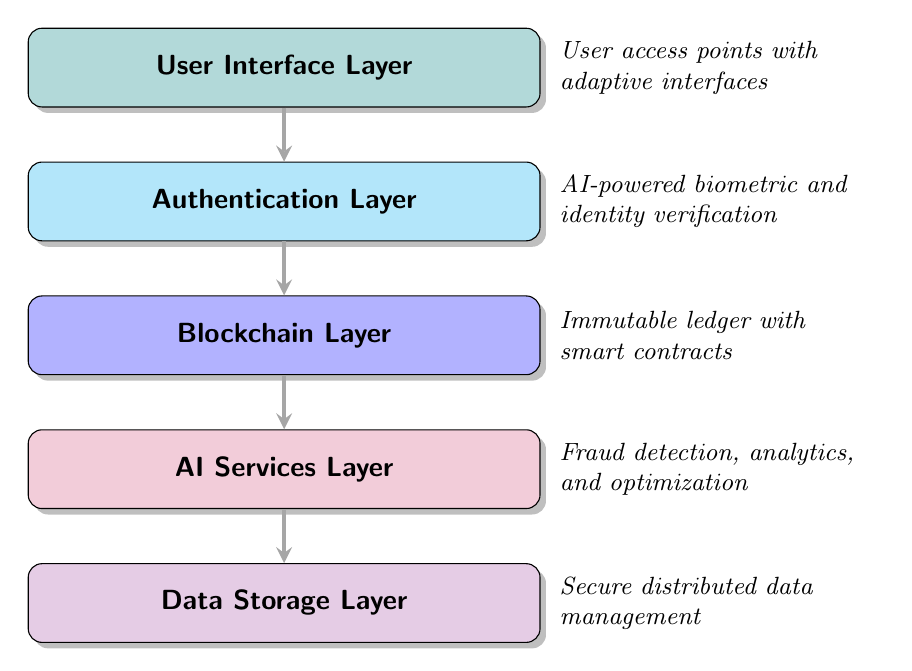
\begin{tikzpicture}[
  node distance=0.7cm,
  box/.style={
    draw, 
    fill=blue!10, 
    minimum width=6.5cm, 
    minimum height=1cm, 
    rounded corners=5pt, 
    drop shadow, 
    font=\sffamily\bfseries,
    align=center
  },
  arrow/.style={
    -stealth, 
    line width=1.5pt, 
    draw=gray!70
  }
]
% Layers - enhanced structure with better styling
\node[box, fill=teal!30] (l5) at (0,0) {User Interface Layer};
\node[box, fill=cyan!30] (l4) at (0,-1.7) {Authentication Layer};
\node[box, fill=blue!30] (l3) at (0,-3.4) {Blockchain Layer};
\node[box, fill=purple!20] (l2) at (0,-5.1) {AI Services Layer};
\node[box, fill=violet!20] (l1) at (0,-6.8) {Data Storage Layer};

% Connections with better arrows
\draw[arrow] (l5) -- (l4);
\draw[arrow] (l4) -- (l3);
\draw[arrow] (l3) -- (l2);
\draw[arrow] (l2) -- (l1);

% Add layer descriptions on the right
\node[text width=4cm, align=left, font=\small\itshape] at (5.5,0) {User access points with adaptive interfaces};
\node[text width=4cm, align=left, font=\small\itshape] at (5.5,-1.7) {AI-powered biometric and identity verification};
\node[text width=4cm, align=left, font=\small\itshape] at (5.5,-3.4) {Immutable ledger with smart contracts};
\node[text width=4cm, align=left, font=\small\itshape] at (5.5,-5.1) {Fraud detection, analytics, and optimization};
\node[text width=4cm, align=left, font=\small\itshape] at (5.5,-6.8) {Secure distributed data management};
\end{tikzpicture}
\caption{Layered Architecture for AI-Blockchain Voting System}
\label{fig:architecture}
\end{figure}

\subsubsection{User Interface Layer}
The User Interface Layer represents a novel approach to voter interaction through AI-powered adaptive interfaces—a capability absent in current blockchain voting systems. Unlike existing static interfaces, this layer would incorporate machine learning algorithms that dynamically adjust the presentation and interaction models based on user capabilities and preferences, providing unprecedented accessibility for diverse voter populations.

\subsubsection{Authentication Layer}
The Authentication Layer introduces AI-powered verification capabilities not found in current blockchain voting systems. This layer would leverage advanced computer vision and biometric analysis to verify voter identity with sophisticated liveness detection and anti-spoofing measures—significantly advancing beyond the simplistic authentication mechanisms in existing systems. The integration with blockchain-based zero-knowledge proofs represents a new approach to verifying eligibility without exposing personal data.

\subsubsection{Blockchain Layer}
The Blockchain Layer provides the secure, transparent, and immutable foundation for recording votes. While this layer builds upon existing blockchain capabilities, the integration with AI introduces novel enhancements including intelligent contract verification, dynamic consensus optimization, and adaptive security measures—features absent in current blockchain voting implementations that typically operate with static parameters and fixed security models.

\subsubsection{AI Services Layer}
The AI Services Layer introduces transformative intelligent capabilities missing from current blockchain voting systems. This new layer would incorporate fraud detection algorithms that analyze patterns in real-time, optimization models that enhance system performance, anomaly detection to identify security threats, and predictive analytics for resource allocation—all representing significant advances beyond the limited analytical capabilities of existing blockchain voting platforms.

\subsubsection{Data Storage Layer}
The Data Storage Layer enhances data management beyond current blockchain systems through AI integration. This layer would incorporate intelligent data routing, automated backup strategies, and optimized storage allocation—adaptive capabilities not present in existing blockchain voting systems that typically employ static data management approaches.

\section{AI-Blockchain Integration Points}
Our framework identifies pioneering integration points where AI and blockchain technologies could synergistically enhance voting systems—combinations that remain unexplored in current implementations. Figures~\ref{fig:integration} and~\ref{fig:workflow} illustrate these novel integration points and their information flows.

\begin{figure}[!htb]
\centering
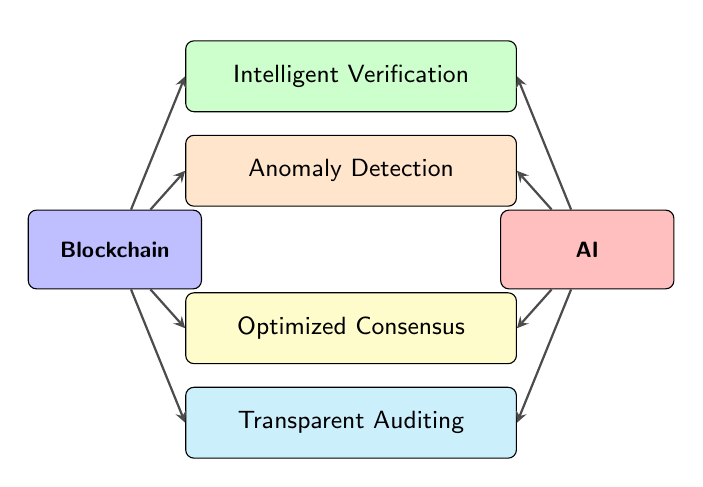
\begin{tikzpicture}[
  node distance=1.4cm,
  tech/.style={
    rectangle, 
    draw=black, 
    fill=#1!25, 
    minimum width=2.2cm, 
    minimum height=1cm, 
    rounded corners=3pt,
    font=\sffamily\bfseries\footnotesize,
    align=center
  },
  integration/.style={
    rectangle, 
    draw=black, 
    fill=#1!20, 
    minimum width=4.2cm, 
    minimum height=0.9cm, 
    rounded corners=3pt,
    font=\sffamily\small,
    align=center
  },
  connection/.style={
    -stealth, 
    thick, 
    draw=black!70
  }
]

% Left and right main technologies
\node[tech=blue] (bc) at (0,0) {Blockchain};
\node[tech=red] (ai) at (6,0) {AI};

% Middle stack
\node[integration=green] (iv) at (3,2.2) {Intelligent Verification};
\node[integration=orange] (ad) at (3,1) {Anomaly Detection};
\node[integration=yellow] (oc) at (3,-1) {Optimized Consensus};
\node[integration=cyan] (ta) at (3,-2.2) {Transparent Auditing};

% Arrows from tech to integration
\draw[connection] (bc) -- (iv.west);
\draw[connection] (ai) -- (iv.east);

\draw[connection] (bc) -- (ad.west);
\draw[connection] (ai) -- (ad.east);

\draw[connection] (bc) -- (oc.west);
\draw[connection] (ai) -- (oc.east);

\draw[connection] (bc) -- (ta.west);
\draw[connection] (ai) -- (ta.east);

% Feature label
\node[font=\scriptsize, anchor=west] at (0,2.7) {};

\end{tikzpicture}
\caption{Integration points between AI and blockchain technologies in voting systems}
\label{fig:integration}
\end{figure}

\subsubsection{Intelligent Verification}
This novel integration point combines AI-powered identity verification technologies with blockchain-based zero-knowledge proofs—a combination not implemented in current voting systems. Unlike existing verification methods that either lack biometric sophistication or privacy guarantees, this approach would enable secure authentication that leverages the pattern-recognition capabilities of AI while maintaining the cryptographic privacy protections of blockchain.

\subsubsection{Anomaly Detection}
The Anomaly Detection integration represents a new capability for voting systems by combining AI fraud detection algorithms with blockchain's immutable record. This unexplored combination would enable identification of suspicious patterns and behaviors before votes are permanently recorded—a preventive capability absent from current blockchain voting systems that typically lack real-time anomaly detection.

\subsubsection{Optimized Consensus}
This integration point introduces a transformative capability through AI-optimized blockchain consensus—a feature missing from existing voting systems. Current blockchain voting platforms operate with static consensus parameters, whereas this novel approach would use AI to dynamically adjust these parameters based on network conditions, voting patterns, and system performance—addressing the critical scalability challenges that limit current systems.

\subsubsection{Transparent Auditing}
The Transparent Auditing integration point combines blockchain's transparent record with AI's analytical capabilities to create novel audit processes not present in current systems. Unlike existing blockchain voting platforms that typically require manual analysis for identifying anomalies, this approach would leverage AI to detect statistical irregularities while leveraging blockchain to ensure the audit process itself remains transparent and verifiable.

\subsection{Information Flow and System Processes}
The conceptual framework includes novel processes that span multiple layers and components, representing a workflow not implemented in current systems. Fig. 3 illustrates a high-level view of information flow through the integrated system, highlighting the role of both AI and blockchain components.

\begin{figure}[!htb]
\raggedright
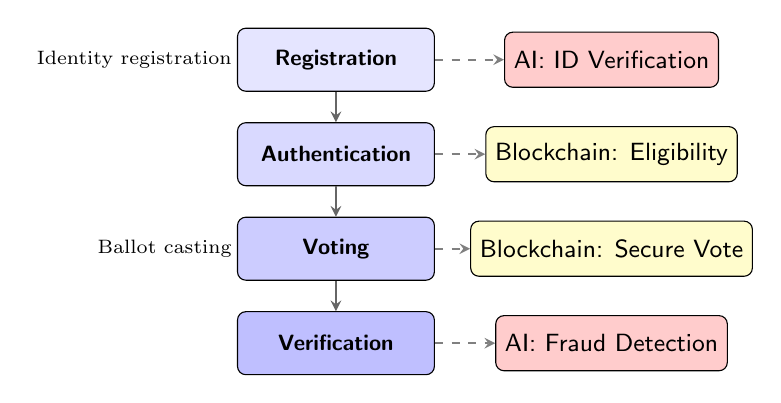
\begin{tikzpicture}[
  node distance=1.5cm,
  process/.style={
    rectangle, 
    draw=black, 
    fill=blue!#1, 
    minimum width=2.5cm, 
    minimum height=0.8cm, 
    rounded corners=3pt,
    font=\sffamily\bfseries\footnotesize,
    align=left
  },
  tech/.style={
    rectangle, 
    draw=black, 
    fill=#1!20, 
    minimum width=2.5cm, 
    minimum height=0.7cm, 
    rounded corners=3pt,
    font=\sffamily\small,
    align=left
  },
  flow/.style={
    -stealth, 
    line width=0.7pt, 
    draw=black!60
  },
  dashflow/.style={
    -stealth, 
    line width=0.7pt, 
    draw=black!50, 
    dashed
  }
]
% Process flow
\node[process=10] (reg) at (0,0) {Registration};
\node[process=15] (auth) at (0,-1.2) {Authentication};
\node[process=20] (vote) at (0,-2.4) {Voting};
\node[process=25] (verify) at (0,-3.6) {Verification};

% Technology
\node[tech=red] (ai1) at (3.5,0) {AI: ID Verification};
\node[tech=yellow] (bc1) at (3.5,-1.2) {Blockchain: Eligibility};
\node[tech=yellow] (bc2) at (3.5,-2.4) {Blockchain: Secure Vote};
\node[tech=red] (ai2) at (3.5,-3.6) {AI: Fraud Detection};

% Connections
\draw[flow] (reg) -- (auth);
\draw[flow] (auth) -- (vote);
\draw[flow] (vote) -- (verify);

\draw[dashflow] (reg) -- (ai1);
\draw[dashflow] (auth) -- (bc1);
\draw[dashflow] (vote) -- (bc2);
\draw[dashflow] (verify) -- (ai2);

% Descriptions
\node[font=\scriptsize, anchor=east] at (-1.2,0) {Identity registration};
\node[font=\scriptsize, anchor=east] at (-1.2,-2.4) {Ballot casting};
\end{tikzpicture}
\caption{Information flow in AI-blockchain voting system}
\label{fig:workflow}
\end{figure}

This information flow represents a novel conceptual process that integrates AI and blockchain components across various phases of the electoral process—a combination not present in current implementations. Unlike existing blockchain voting systems that lack intelligent components, this framework envisions a cohesive workflow where AI and blockchain capabilities complement each other throughout the voting lifecycle, from registration to result verification.

\section{Novel Applications of AI in Blockchain Voting}
Based on our conceptual framework, we identify several groundbreaking applications for AI integration in blockchain voting systems. These represent innovations not currently implemented in existing systems but that could address critical challenges in electronic voting.

\subsection{Intelligent Authentication and Verification}
The integration of AI-powered biometric authentication with blockchain-based eligibility verification represents a novel approach absent from current voting systems. This unprecedented combination would transform voter authentication through:

\begin{itemize}
    \item \textbf{Multi-modal biometric verification:} A new capability that would combine facial recognition, fingerprint scanning, and potentially voice recognition through advanced neural network models to achieve significantly higher accuracy than the single-factor approaches used in current systems.
    
    \item \textbf{Document verification:} An innovative application using computer vision and OCR technologies to authenticate identification documents in real-time—a capability missing from current blockchain voting systems that typically rely on pre-registration of static credentials.
    
    \item \textbf{Behavioral biometrics:} A pioneering security layer that would analyze typing patterns, gesture dynamics, or other behavioral markers as an additional verification mechanism—particularly valuable for remote voting scenarios where traditional authentication methods are vulnerable.
    
    \item \textbf{Zero-knowledge eligibility proofs:} A novel cryptographic approach recorded on the blockchain that would verify a voter's eligibility without revealing their identity—creating a privacy-preserving yet verifiable authentication process not available in current systems.
\end{itemize}

These capabilities would transform the fundamental challenge of voter authentication in electronic systems—moving beyond the simplistic verification mechanisms in current blockchain voting platforms to create a system that provides strong security while maintaining privacy and accessibility.

\subsection{AI-Powered Fraud Detection and Prevention}
The integration of AI with blockchain for fraud detection represents a transformative capability not present in current voting systems:

\begin{itemize}
    \item \textbf{Real-time anomaly detection:} A groundbreaking application where machine learning algorithms would analyze voting patterns and system interactions to identify statistical outliers that might indicate fraud attempts—a proactive capability absent from current blockchain voting systems that typically rely on post-election analysis.
    
    \item \textbf{Duplicate vote prevention:} An innovative combination of blockchain's consensus mechanisms with AI detection systems to ensure each eligible voter can cast only one valid vote—providing a more sophisticated approach than the simple token-based methods in current systems.
    
    \item \textbf{Smart contract monitoring:} A novel security measure where AI systems would continuously monitor smart contract execution to detect potential exploits or unexpected behaviors—identifying sophisticated attacks that might bypass the static security checks in current blockchain voting platforms.
    
    \item \textbf{Network security:} A pioneering application of AI-powered intrusion detection systems to protect blockchain nodes from denial-of-service attacks or unauthorized access attempts during critical voting periods—a dynamic defense capability missing from current systems.
\end{itemize}

These applications would establish a new paradigm for election security by combining the immutable record-keeping of blockchain with the pattern recognition and predictive capabilities of AI—creating a system that can anticipate and prevent electoral fraud rather than merely recording it.

\subsection{Adaptive User Interfaces and Accessibility}
AI integration would enable unprecedented accessibility enhancements in blockchain voting systems through:

\begin{itemize}
    \item \textbf{Adaptive interfaces:} A transformative capability where machine learning algorithms would adjust the user interface based on user capabilities, preferences, and device characteristics—making the system more accessible to voters with different needs than the static interfaces in current blockchain voting platforms.
    
    \item \textbf{Natural language processing:} An innovative application enabling voice-controlled interfaces and multilingual support—reducing barriers for voters with limited literacy or physical disabilities in ways not addressed by current blockchain voting systems.
    
    \item \textbf{Personalized assistance:} A novel support mechanism where AI chatbots or virtual assistants would guide voters through the registration and voting process—providing context-specific help without compromising ballot secrecy, unlike the generic help systems in current platforms.
    
    \item \textbf{Accessibility verification:} A pioneering quality assurance approach where AI systems would automatically test voting interfaces against accessibility standards—identifying and suggesting improvements to ensure compliance with accessibility requirements.
\end{itemize}

These applications would address a critical gap in current blockchain voting systems: accessibility and usability for diverse voter populations. By leveraging AI to enhance the user experience, these systems would become more inclusive while maintaining the security benefits of blockchain—a combination not effectively implemented in existing platforms.

\subsection{Transparent AI-Enhanced Auditing}
The combination of AI analytics with blockchain's immutable record would create revolutionary tools for election integrity not found in current systems:

\begin{itemize}
    \item \textbf{Statistical verification:} A novel analytical capability where machine learning models would analyze voting results to identify statistically improbable patterns that might indicate manipulation or system errors—with the blockchain providing a transparent record of these analyses unlike the manual, ad-hoc auditing in current systems.
    
    \item \textbf{Automated auditing:} A groundbreaking application where AI would automate parts of the post-election audit process—analyzing the blockchain record to verify that all votes were properly recorded and counted without revealing individual vote choices, a capability absent from current blockchain voting platforms.
    
    \item \textbf{Explainable verification:} A pioneering approach where AI systems would generate human-understandable explanations of verification processes—helping voters, officials, and observers understand how the integrity of the election was maintained, addressing the "black box" perception of current blockchain systems.
    
    \item \textbf{Continuous monitoring:} An innovative shift from post-election audits to continuous monitoring of the voting system—where AI would identify and address potential issues in real-time while recording these actions on the blockchain for transparency, a proactive approach not implemented in current systems.
\end{itemize}

These applications would transform election verification by combining the analytical power of AI with the transparency and immutability of blockchain—addressing the critical need for public trust in electronic voting systems through capabilities not present in current blockchain voting platforms.

\subsection{Dynamic Consensus Optimization}
A revolutionary application of AI to blockchain voting would be the dynamic optimization of consensus mechanisms—a capability entirely absent from current systems:

\begin{itemize}
    \item \textbf{Adaptive consensus parameters:} A novel approach where machine learning algorithms would dynamically adjust blockchain consensus parameters based on current network conditions, voting volume, and threat assessments—optimizing performance and security in ways not possible with the static configurations in current blockchain voting systems.
    
    \item \textbf{Predictive resource allocation:} An innovative capability where AI would forecast voting patterns and system demands to proactively allocate computational resources—preventing bottlenecks during peak voting periods unlike the fixed resource allocation in current blockchain implementations.
    
    \item \textbf{Distributed denial-of-service (DDoS) resilience:} A pioneering security enhancement where AI would detect potential DDoS attacks and dynamically adjust network configurations to maintain system availability—providing adaptive protection not present in current blockchain voting platforms.
    
    \item \textbf{Energy-efficient operation:} A transformative approach where machine learning would optimize consensus mechanisms to minimize energy consumption while maintaining security—addressing the sustainability concerns of blockchain voting in ways not implemented in current systems.
\end{itemize}

These applications would resolve one of the fundamental limitations of current blockchain voting systems—scalability and performance during large-scale elections—through the novel application of AI to dynamically optimize system operations based on real-time conditions.

\subsection{Privacy-Preserving Analytics}
The integration of AI with blockchain would enable unprecedented privacy-preserving analytics capabilities not found in current voting systems:

\begin{itemize}
    \item \textbf{Differential privacy implementation:} A novel approach where AI would dynamically adjust privacy parameters when analyzing voting data—ensuring statistical utility while mathematically guaranteeing individual voter privacy, a sophisticated capability absent from current blockchain voting platforms.
    
    \item \textbf{Encrypted analysis techniques:} An innovative application where machine learning models would operate on encrypted data without decryption—enabling powerful analytics while maintaining ballot secrecy, unlike the limited analytics in current systems that require privacy compromises.
    
    \item \textbf{Federated learning for voting patterns:} A groundbreaking implementation where AI models would learn from distributed voting data without centralizing sensitive information—creating insights while preserving privacy in ways not possible with current blockchain analytics.
    
    \item \textbf{Privacy risk assessment:} A pioneering protection mechanism where AI would continuously evaluate the risk of de-anonymization from published voting statistics—adjusting the granularity of public data to prevent privacy breaches, a dynamic capability missing from current blockchain voting systems.
\end{itemize}

These applications would resolve the tension between valuable electoral analytics and voter privacy through novel AI techniques that maintain strong privacy guarantees while enabling sophisticated analysis—a balance not achieved in current blockchain voting implementations.

\section{Implementation Challenges}
The proposed integration of AI with blockchain for voting systems represents a paradigm shift that would face significant implementation challenges not previously addressed in the literature or practice.

\subsection{Technical Challenges}
The novel integration of AI with blockchain for voting would face several technical hurdles:

\begin{itemize}
    \item \textbf{Scalability limitations:} Blockchain networks face significant throughput constraints compared to traditional databases. While AI could potentially optimize consensus parameters, fundamental blockchain architecture limitations would need to be addressed for large-scale elections with millions of voters in short timeframes—a challenge requiring novel technical solutions beyond current approaches.
    
    \item \textbf{Energy consumption:} Many blockchain consensus mechanisms, particularly Proof-of-Work, consume substantial energy. While AI could help optimize energy usage, the underlying energy intensity of secure blockchain operations presents a significant challenge for sustainable implementation—requiring innovative consensus approaches specifically designed for the voting context.
    
    \item \textbf{Integration complexity:} Effectively integrating AI with blockchain systems would require addressing fundamental differences in processing models, data storage, and system architecture. This unprecedented integration would add significant complexity to system design and implementation—necessitating new architectural patterns and integration frameworks not currently established in either field.
    
    \item \textbf{AI model security:} AI models themselves can be vulnerable to adversarial attacks, where specially crafted inputs cause the model to make incorrect predictions. For voting applications, such vulnerabilities could compromise critical functions like voter authentication or fraud detection—requiring novel approaches to AI security not widely implemented in current systems.
    
    \item \textbf{Consensus mechanism selection:} Choosing appropriate consensus mechanisms for AI-enhanced voting systems would involve complex trade-offs between security, performance, and energy efficiency—requiring new evaluation frameworks specifically designed for this novel integration.
\end{itemize}

\subsection{Data Privacy and Security Concerns}
The proposed AI-blockchain integration would present unprecedented privacy and security challenges:

\begin{itemize}
    \item \textbf{Biometric data protection:} AI-powered authentication would rely on sensitive biometric data. Storing and processing this data securely while maintaining its usefulness for verification presents significant privacy challenges not fully resolved in current biometric systems—requiring novel approaches to privacy-preserving biometric processing.
    
    \item \textbf{Blockchain privacy limitations:} While blockchains provide transparency, excessive transparency can compromise voter privacy. Techniques like zero-knowledge proofs and homomorphic encryption add complexity and processing overhead—creating implementation challenges not addressed in current blockchain voting platforms.
    
    \item \textbf{Re-identification risks:} Even with privacy-preserving techniques, the combination of multiple data points recorded on the blockchain might allow for voter re-identification through sophisticated analysis—presenting novel privacy challenges requiring advanced protection mechanisms not implemented in current systems.
    
    \item \textbf{Data management across borders:} International or diaspora voting introduces questions about data sovereignty and cross-border data transfers, particularly for sensitive biometric information used in AI authentication—presenting regulatory and technical challenges not addressed in current voting platforms.
\end{itemize}

\subsection{Regulatory and Legal Challenges}
The implementation of AI-blockchain voting systems would face unprecedented regulatory and legal hurdles:

\begin{itemize}
    \item \textbf{Regulatory uncertainty:} Many jurisdictions lack comprehensive regulatory frameworks for either blockchain-based voting or AI in electoral systems, creating legal uncertainty for implementation—requiring novel regulatory approaches specifically designed for this integrated technology.
    
    \item \textbf{Compliance with electoral laws:} Existing electoral laws were generally written with paper-based voting in mind and may not easily accommodate the novel combination of AI and blockchain technologies without legislative updates—necessitating new legal frameworks for electronic voting.
    
    \item \textbf{Certification standards:} The lack of established certification standards specifically for AI-blockchain voting systems would make it difficult to validate their security, reliability, and compliance with electoral requirements—requiring new certification methodologies not currently available.
    
    \item \textbf{Liability and accountability:} Determining responsibility when issues arise in AI-driven decisions or blockchain-based recording presents complex legal questions that current frameworks may not adequately address—requiring novel approaches to technological accountability in electoral systems.
\end{itemize}

\subsection{Ethical and Social Considerations}
Beyond technical and legal challenges, the novel integration of AI with blockchain for voting would raise important ethical and social questions:

\begin{itemize}
    \item \textbf{Digital divide:} AI-enhanced blockchain solutions might disadvantage voters without access to or familiarity with required devices and interfaces, potentially disenfranchising portions of the electorate—presenting ethical challenges not resolved in current digital voting approaches.
    
    \item \textbf{Algorithmic bias:} AI systems may exhibit bias in authentication or fraud detection across demographic groups if not properly designed and tested with diverse data—presenting novel ethical concerns requiring specialized approaches to fair AI in electoral contexts.
    
    \item \textbf{Transparency vs. comprehensibility:} While blockchain provides technical transparency, both blockchain and AI technologies may appear as "black boxes" to most voters, potentially undermining trust rather than enhancing it—requiring innovative approaches to explainable AI not widely implemented in current systems.
    
    \item \textbf{Democratic oversight:} Determining who controls, audits, and certifies these novel integrated systems raises fundamental questions about democratic oversight and the role of technology in electoral processes—requiring new governance models not established in current voting platforms.
    
    \item \textbf{Coercion in remote voting:} Remote voting, even with AI and blockchain security measures, would remain vulnerable to coercion in unsupervised environments—presenting social challenges requiring novel approaches beyond technological solutions.
\end{itemize}

These challenges highlight the need for careful, interdisciplinary approaches to AI-blockchain integration in voting that consider not only technical feasibility but also legal compliance, ethical implications, and social impact—a comprehensive perspective not yet developed for this novel technological combination.

\section{Research Directions for AI-Blockchain Voting}
Based on our analysis of the potential for AI-blockchain integration in voting systems and the identified challenges, we propose several pioneering research directions to advance this new field.

\subsection{Technical Research Opportunities}
Several technical areas require foundational research to realize the potential of AI-blockchain integration in voting systems:

\begin{itemize}
    \item \textbf{Scalable AI-optimized blockchain architectures:} Developing high-throughput blockchain architectures specifically designed for voting applications, where AI dynamically manages sharding, consensus participant selection, and transaction propagation—representing a novel technical approach not explored in current blockchain systems.
    
    \item \textbf{Privacy-preserving AI for biometrics:} Creating new techniques for AI to process biometric data without compromising privacy, including federated learning models that never centralize sensitive information and zero-knowledge proofs for biometric matching—innovations not implemented in current authentication systems.
    
    \item \textbf{Adversarial-resistant voting AI:} Developing AI models specifically resistant to electoral fraud attempts, ensuring that authentication and fraud detection systems cannot be manipulated through specially crafted inputs—a specialized security approach not addressed in current AI literature.
    
    \item \textbf{On-chain AI verification:} Creating novel mechanisms for blockchain-based verification of AI model integrity and decision processes, ensuring that the AI components cannot be tampered with and their operations remain transparent—a verification capability not implemented in current systems.
    
    \item \textbf{Cross-chain AI coordination:} Developing new approaches for AI to coordinate voting processes across multiple blockchain networks, enabling higher throughput and resilience through intelligently managed cross-chain operations—a capability not explored in current blockchain voting.
\end{itemize}

\subsection{Novel System Integration and Standards}
Standardization and integration frameworks represent crucial areas for establishing this new field:

\begin{itemize}
    \item \textbf{Reference architectures:} Developing the first open reference architectures for integrating AI with blockchain in voting applications, providing guidelines for component interaction, data flow, and security requirements—establishing a foundation for this novel technological combination.
    
    \item \textbf{Interoperability standards:} Creating new standards for data exchange between AI and blockchain components, enabling different implementations to work together cohesively and facilitating modular system design—providing an integration framework not currently available.
    
    \item \textbf{Testing and certification methodologies:} Establishing comprehensive testing approaches specifically for AI-blockchain voting systems, addressing their unique characteristics and risk profiles—creating evaluation methods not present in current certification frameworks.
    
    \item \textbf{Benchmarking datasets and environments:} Creating standardized, diverse datasets for training and testing AI components of voting systems, particularly for authentication and fraud detection—establishing resources not currently available for this novel application domain.
\end{itemize}

\subsection{Implementation and Governance Research}
Research on practical implementation and governance models would be essential for real-world applications of this novel technology:

\begin{itemize}
    \item \textbf{Multi-stakeholder governance models:} Developing and evaluating new governance frameworks for AI-blockchain voting systems that balance technical expertise, democratic oversight, and public accountability in system management—creating approaches not established in current electronic voting.
    
    \item \textbf{Progressive implementation strategies:} Researching novel approaches for gradual adoption, such as using AI-blockchain systems alongside traditional methods before full transition—developing transition methodologies not explored in current voting literature.
    
    \item \textbf{Cross-border implementation:} Studying the legal, technical, and operational challenges of implementing these novel systems across jurisdictional boundaries for international or diaspora voting—addressing governance questions not resolved in current electronic voting.
    
    \item \textbf{Comprehensive risk assessment frameworks:} Creating new methodologies for assessing the security, privacy, and social risks of AI-blockchain voting implementations in different contexts—establishing evaluation approaches not available for this integrated technology.
\end{itemize}

\subsection{Human Factors and Accessibility Research}
Understanding human interaction with these novel systems represents a critical research area:

\begin{itemize}
    \item \textbf{Universal design approaches:} Researching new design methodologies that ensure AI-blockchain voting systems are accessible to all voters, including those with disabilities, limited technological literacy, or language barriers—creating inclusive approaches not established in current blockchain voting.
    
    \item \textbf{Trust formation studies:} Investigating how voters form trust judgments about AI-blockchain voting systems and identifying design features that enhance legitimate trust—exploring psychological aspects not addressed in current electronic voting research.
    
    \item \textbf{Usability across demographics:} Studying how different demographic groups interact with these novel systems and developing adaptive interfaces that accommodate diverse needs without compromising security or privacy—addressing inclusivity challenges not resolved in current platforms.
    
    \item \textbf{Voter education strategies:} Researching effective approaches for educating voters about AI-blockchain voting systems, balancing technical accuracy with comprehensibility—developing communication frameworks not established for this novel technology.
\end{itemize}

\subsection{Ethical and Societal Impact Research}
Research on ethical implications and societal impacts would be crucial for responsible development of this new technology:

\begin{itemize}
    \item \textbf{Algorithmic fairness in voting:} Developing methodologies for identifying and mitigating bias in AI components of voting systems, with particular attention to authentication and fraud detection algorithms—creating equity approaches not established in current electronic voting.
    
    \item \textbf{Digital divide mitigation:} Researching strategies to ensure AI-blockchain voting systems do not disenfranchise voters with limited technological access or literacy—addressing inclusion challenges not resolved in current blockchain voting platforms.
    
    \item \textbf{Democratic impact assessment:} Developing frameworks to evaluate how AI-blockchain voting systems might affect democratic participation, institutional trust, and civic engagement—exploring societal impacts not examined in current voting technology research.
    
    \item \textbf{Ethical AI in electoral contexts:} Creating specialized ethical guidelines for AI applications in voting systems, addressing the unique requirements and sensitivities of democratic processes—establishing principles not formulated for this novel domain.
\end{itemize}

These research directions would establish the foundation for a new field of AI-blockchain voting systems—addressing critical gaps in current understanding and providing a roadmap for developing electoral technologies that leverage the complementary strengths of these technologies while addressing their limitations.

\section{Conclusion}
This paper has introduced the novel concept of integrating artificial intelligence with blockchain technology to revolutionize electronic voting systems. While blockchain has shown promise for addressing certain aspects of electronic voting, our analysis reveals critical limitations in current implementations that AI could uniquely address—presenting an unprecedented opportunity for technological innovation in electoral systems.

Through a comprehensive analysis of existing blockchain voting platforms, we have identified specific gaps where AI integration could provide transformative capabilities: voter authentication, fraud detection, system optimization, accessibility, and transparent auditing. These areas represent fertile ground for innovation where the pattern recognition, adaptability, and analytical capabilities of AI could complement the immutability, transparency, and decentralization of blockchain.

Our proposed conceptual framework represents the first comprehensive model for AI-blockchain integration in voting systems, illustrating how these technologies could work together across multiple layers and processes. The framework identifies pioneering integration points—intelligent verification, anomaly detection, optimized consensus, and transparent auditing—where AI and blockchain could synergistically enhance electoral integrity, efficiency, and accessibility.

We have proposed several groundbreaking applications for this novel integration, including multi-modal biometric verification, real-time anomaly detection, adaptive user interfaces, automated auditing mechanisms, dynamic consensus optimization, and privacy-preserving analytics. These applications represent significant departures from current blockchain voting systems, which typically operate with static rules and limited intelligence.

While the potential benefits are substantial, we acknowledge that implementing this novel integration would face unprecedented challenges: technical hurdles in scalability and security, privacy concerns around biometric data, regulatory uncertainty in an emerging domain, and ethical questions about technology in democratic processes. These challenges underscore the need for careful, interdisciplinary approaches to development and deployment.

By identifying pioneering research directions—from technical innovations to governance models, human factors, and ethical frameworks—we have established a foundation for a new field of study at the intersection of AI, blockchain, and electoral systems. This research agenda aims to guide the development of technologies that enhance democratic processes rather than undermining them.

The integration of AI with blockchain for voting represents a paradigm shift that could create electoral systems more secure, accessible, and trustworthy than either traditional paper-based methods or current electronic systems. By bringing together these complementary technologies in novel ways, we can address the persistent challenges of digital democracy while safeguarding the fundamental values of electoral integrity, privacy, and accessibility.

This pioneering exploration aims to inspire researchers, practitioners, and policymakers to investigate this untapped potential and collaboratively develop the next generation of voting technologies—systems that leverage the best of human innovation to strengthen democratic institutions in the digital age.

\begin{thebibliography}{8}
\bibitem{b1}
Z. Khudoykulov, U. Tojiakbarova, S. Bozorov and D. Ourbonalieva, ``Blockchain Based E-Voting System: Open Issues and Challenges,'' in {\it International Conference on Information Science and Communications Technologies (ICISCT)}, Tashkent, Uzbekistan, 2021, pp. 1-5, doi: 10.1109/ICISCT52966.2021.9670245.

\bibitem{b2}
A. Balti, A. Prabhu, S. Shahi, S. Dahifale and V. Maheta, ``A Decentralized and Immutable E-Voting System using Blockchain,'' in {\it International Conference on Sustainable Computing and Smart Systems (ICSCSS)}, Coimbatore, India, 2023, pp. 1434-1439, doi: 10.1109/ICSCSS57650.2023.10169552.

\bibitem{b3}
S. Tandon, N. Singh, S. Porwal, Satiram and A. K. Maurya, ``E-Matdaan: A Blockchain based Decentralized E-Voting System,'' in {\it IEEE Students Conference on Engineering and Systems (SCES)}, Prayagraj, India, 2022, pp. 1-6, doi: 10.1109/SCES55490.2022.9887759.

\bibitem{b4}
V. Sliusar, P. Fyodorov, A. Fyodorov, V. Pascari, and A. Volkov, ``Blockchain Technology Application for Electronic Voting Systems,'' in {\it IEEE Conference of Russian Young Researchers in Electrical and Electronic Engineering (ElConRus)}, 2021, pp. 2257-2261, doi: 10.1109/ElConRus51938.2021.9396400.

\bibitem{b5}
S. Singh, A. Singh, S. Verma, and R. K. Dwivedi, ``Designing a Blockchain-Enabled Methodology for Secure Online Voting System,'' in {\it International Conference on Intelligent Data Communication Technologies and Internet of Things (IDCIoT)}, 2023, pp. 178-184, doi: 10.1109/IDCIoT56793.2023.10053410.

\bibitem{b6}
S. Joseph, P. Pandey, M. Khari, K. Kumar, and P. P. Singh, ``Ether Vote: Revolutionizing Elections with Blockchain-Powered Electronic Voting System,'' in {\it 3rd International Conference on Smart Generation Computing, Communication and Networking (SMART GENCON)}, 2023, pp. 1-7, doi: 10.1109/SMARTGENCON60755.2023.10442887.

\bibitem{b7}
J. B. A. Edoo, R. K. Sungkur, J. M. Gómez, H. Precht, and S. Rudolph, ``Mauvote: A Novel Mobile Electronic Voting System Using Blockchain,'' in {\it International Conference on Next Generation Computing Applications (NextComp)}, 2024, pp. 1-6, doi: 10.1109/NextComp63004.2024.10779646.

\bibitem{b8}
N. S. Varma Indukuri, S. Reddy Eguram, A. Nichena, S. Ulvalapudi and R. Gajula, ``Blockchain-based Voting System in a Democratic Environment,'' in {\it Second International Conference on Augmented Intelligence and Sustainable Systems (ICAISS)}, Trichy, India, 2023, pp. 1312-1316, doi: 10.1109/ICAISS58487.2023.10250609.
\end{thebibliography}

\end{document}